\documentclass[main.tex]{subfiles}
\begin{document}
	\begin{figure}[ht]
		\centering
		\begin{subfigure}{0.3\textwidth}
			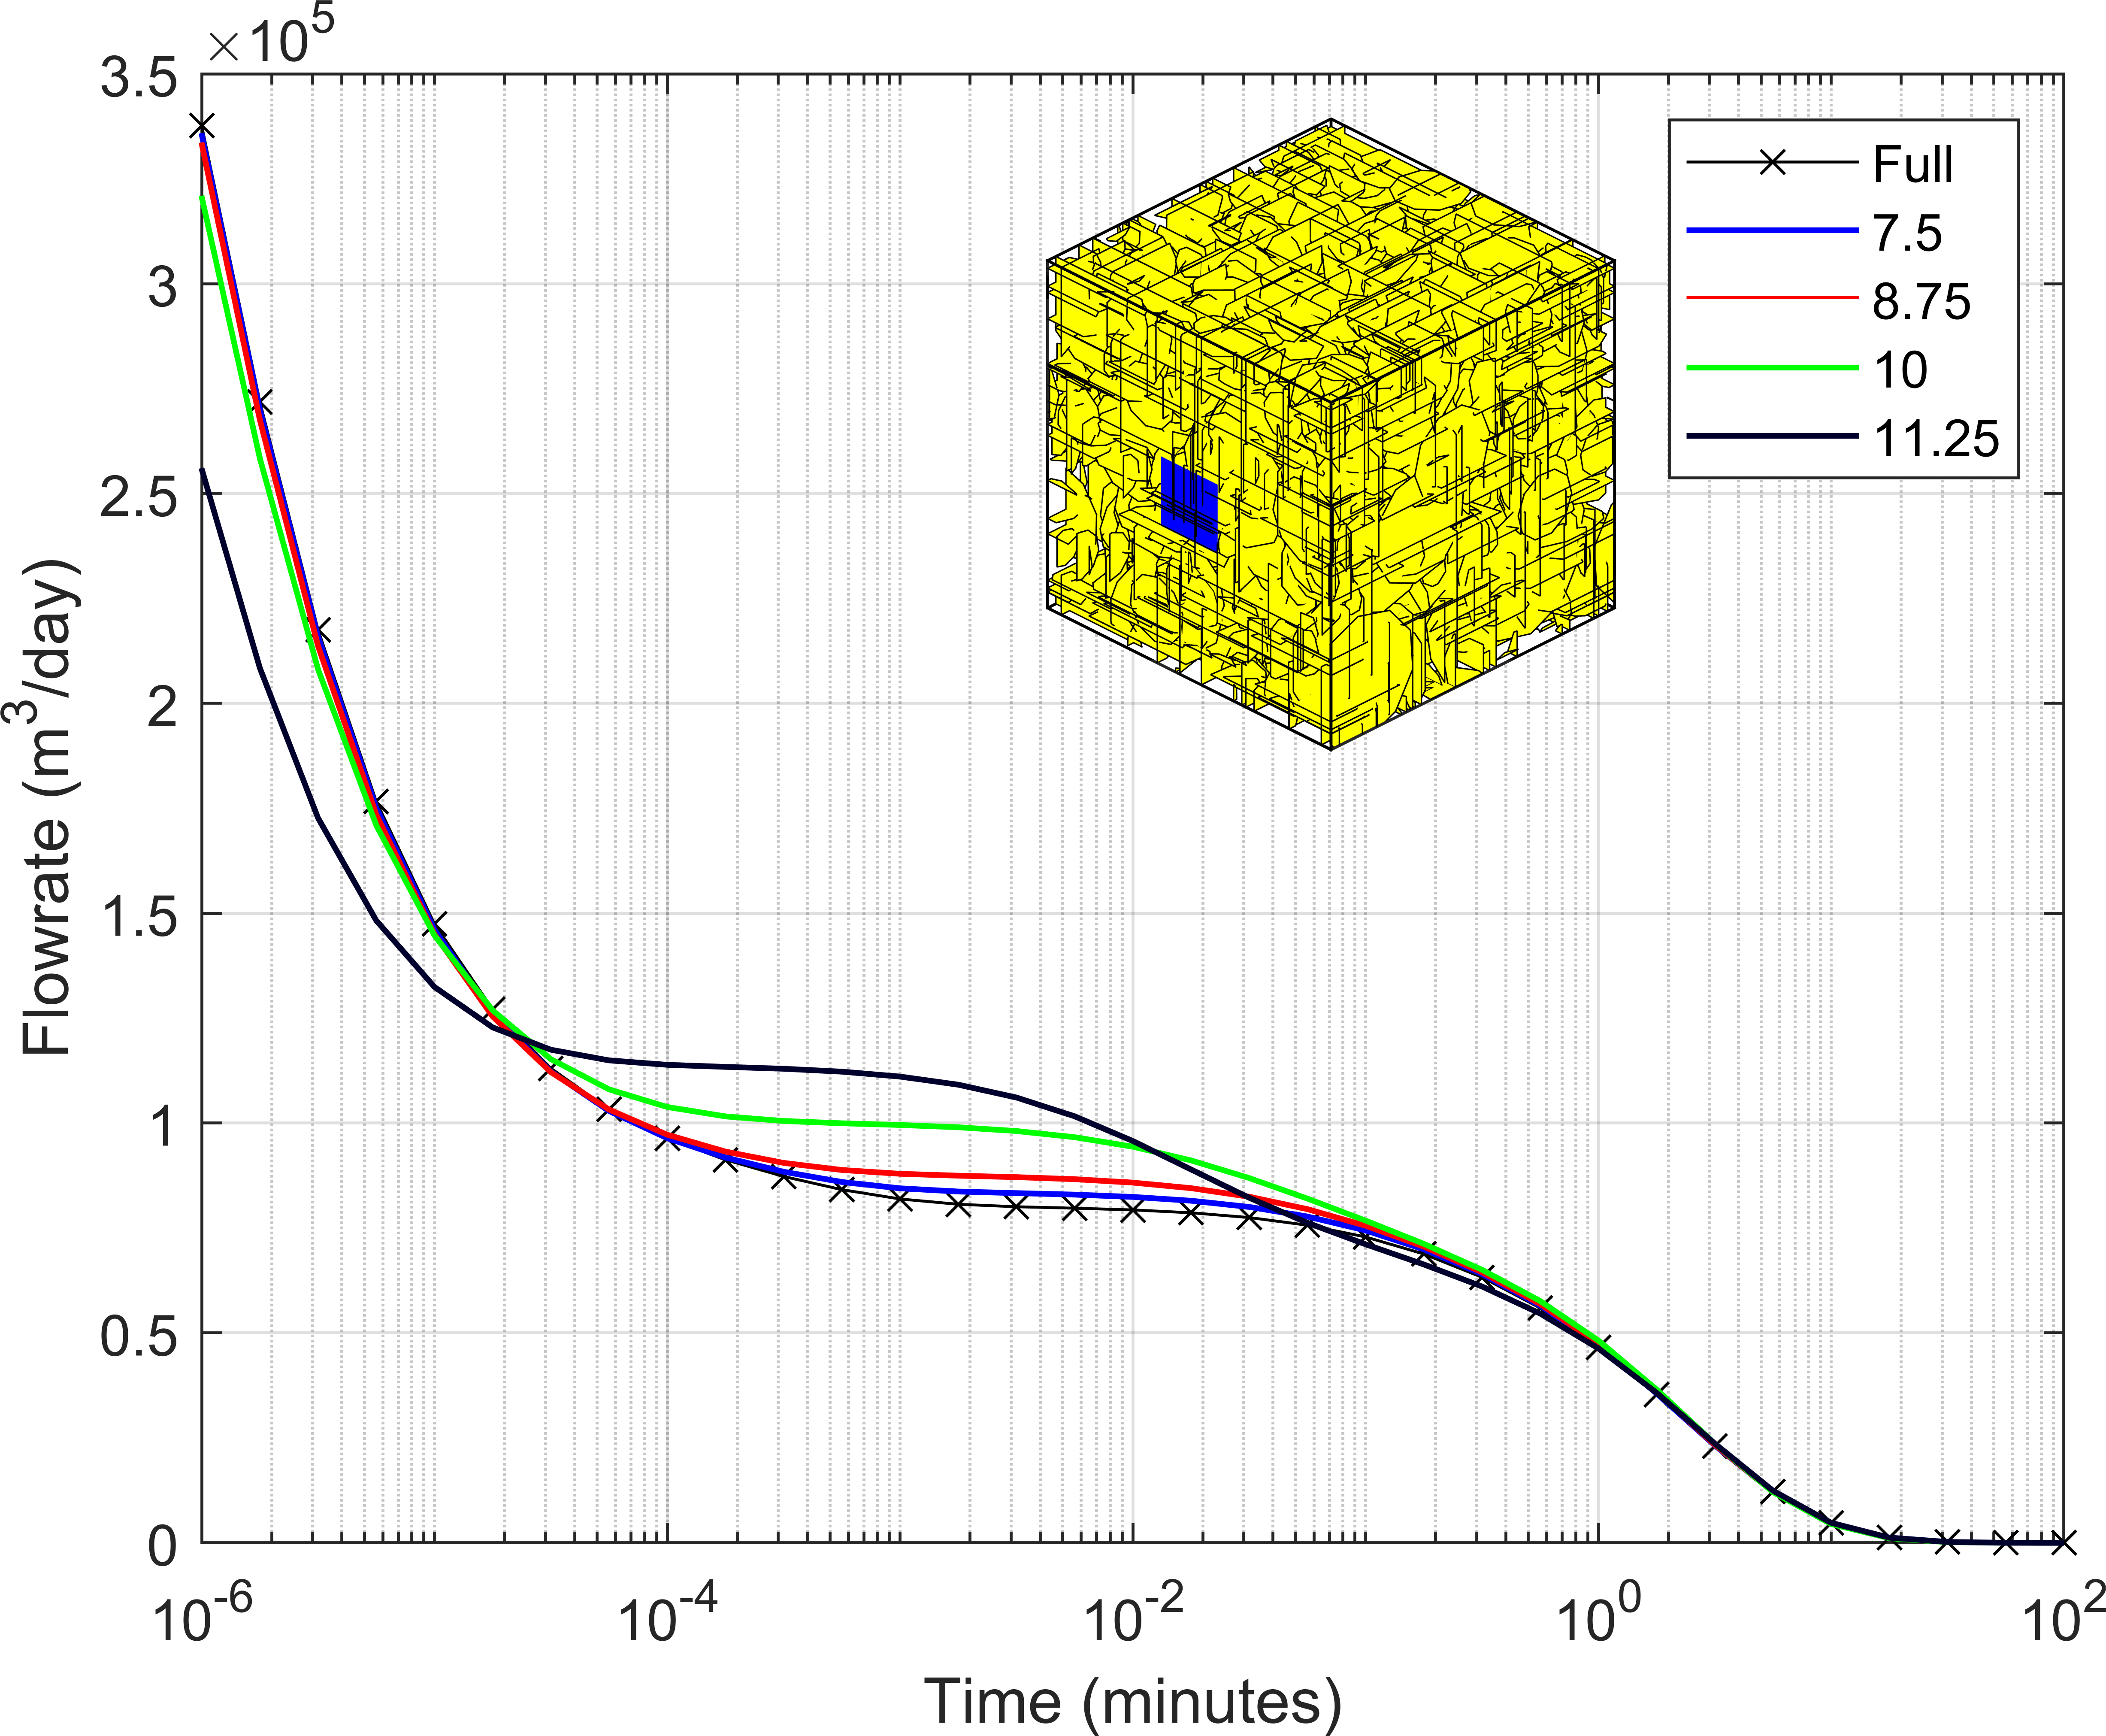
\includegraphics[width=\textwidth]{DD_main/Plot_Drawdown_Case_01_BCinset.png}
			\subcaption{Case A: Base Parameters}
			\label{fig:DD_A}
		\end{subfigure}
		\begin{subfigure}{0.3\textwidth}
			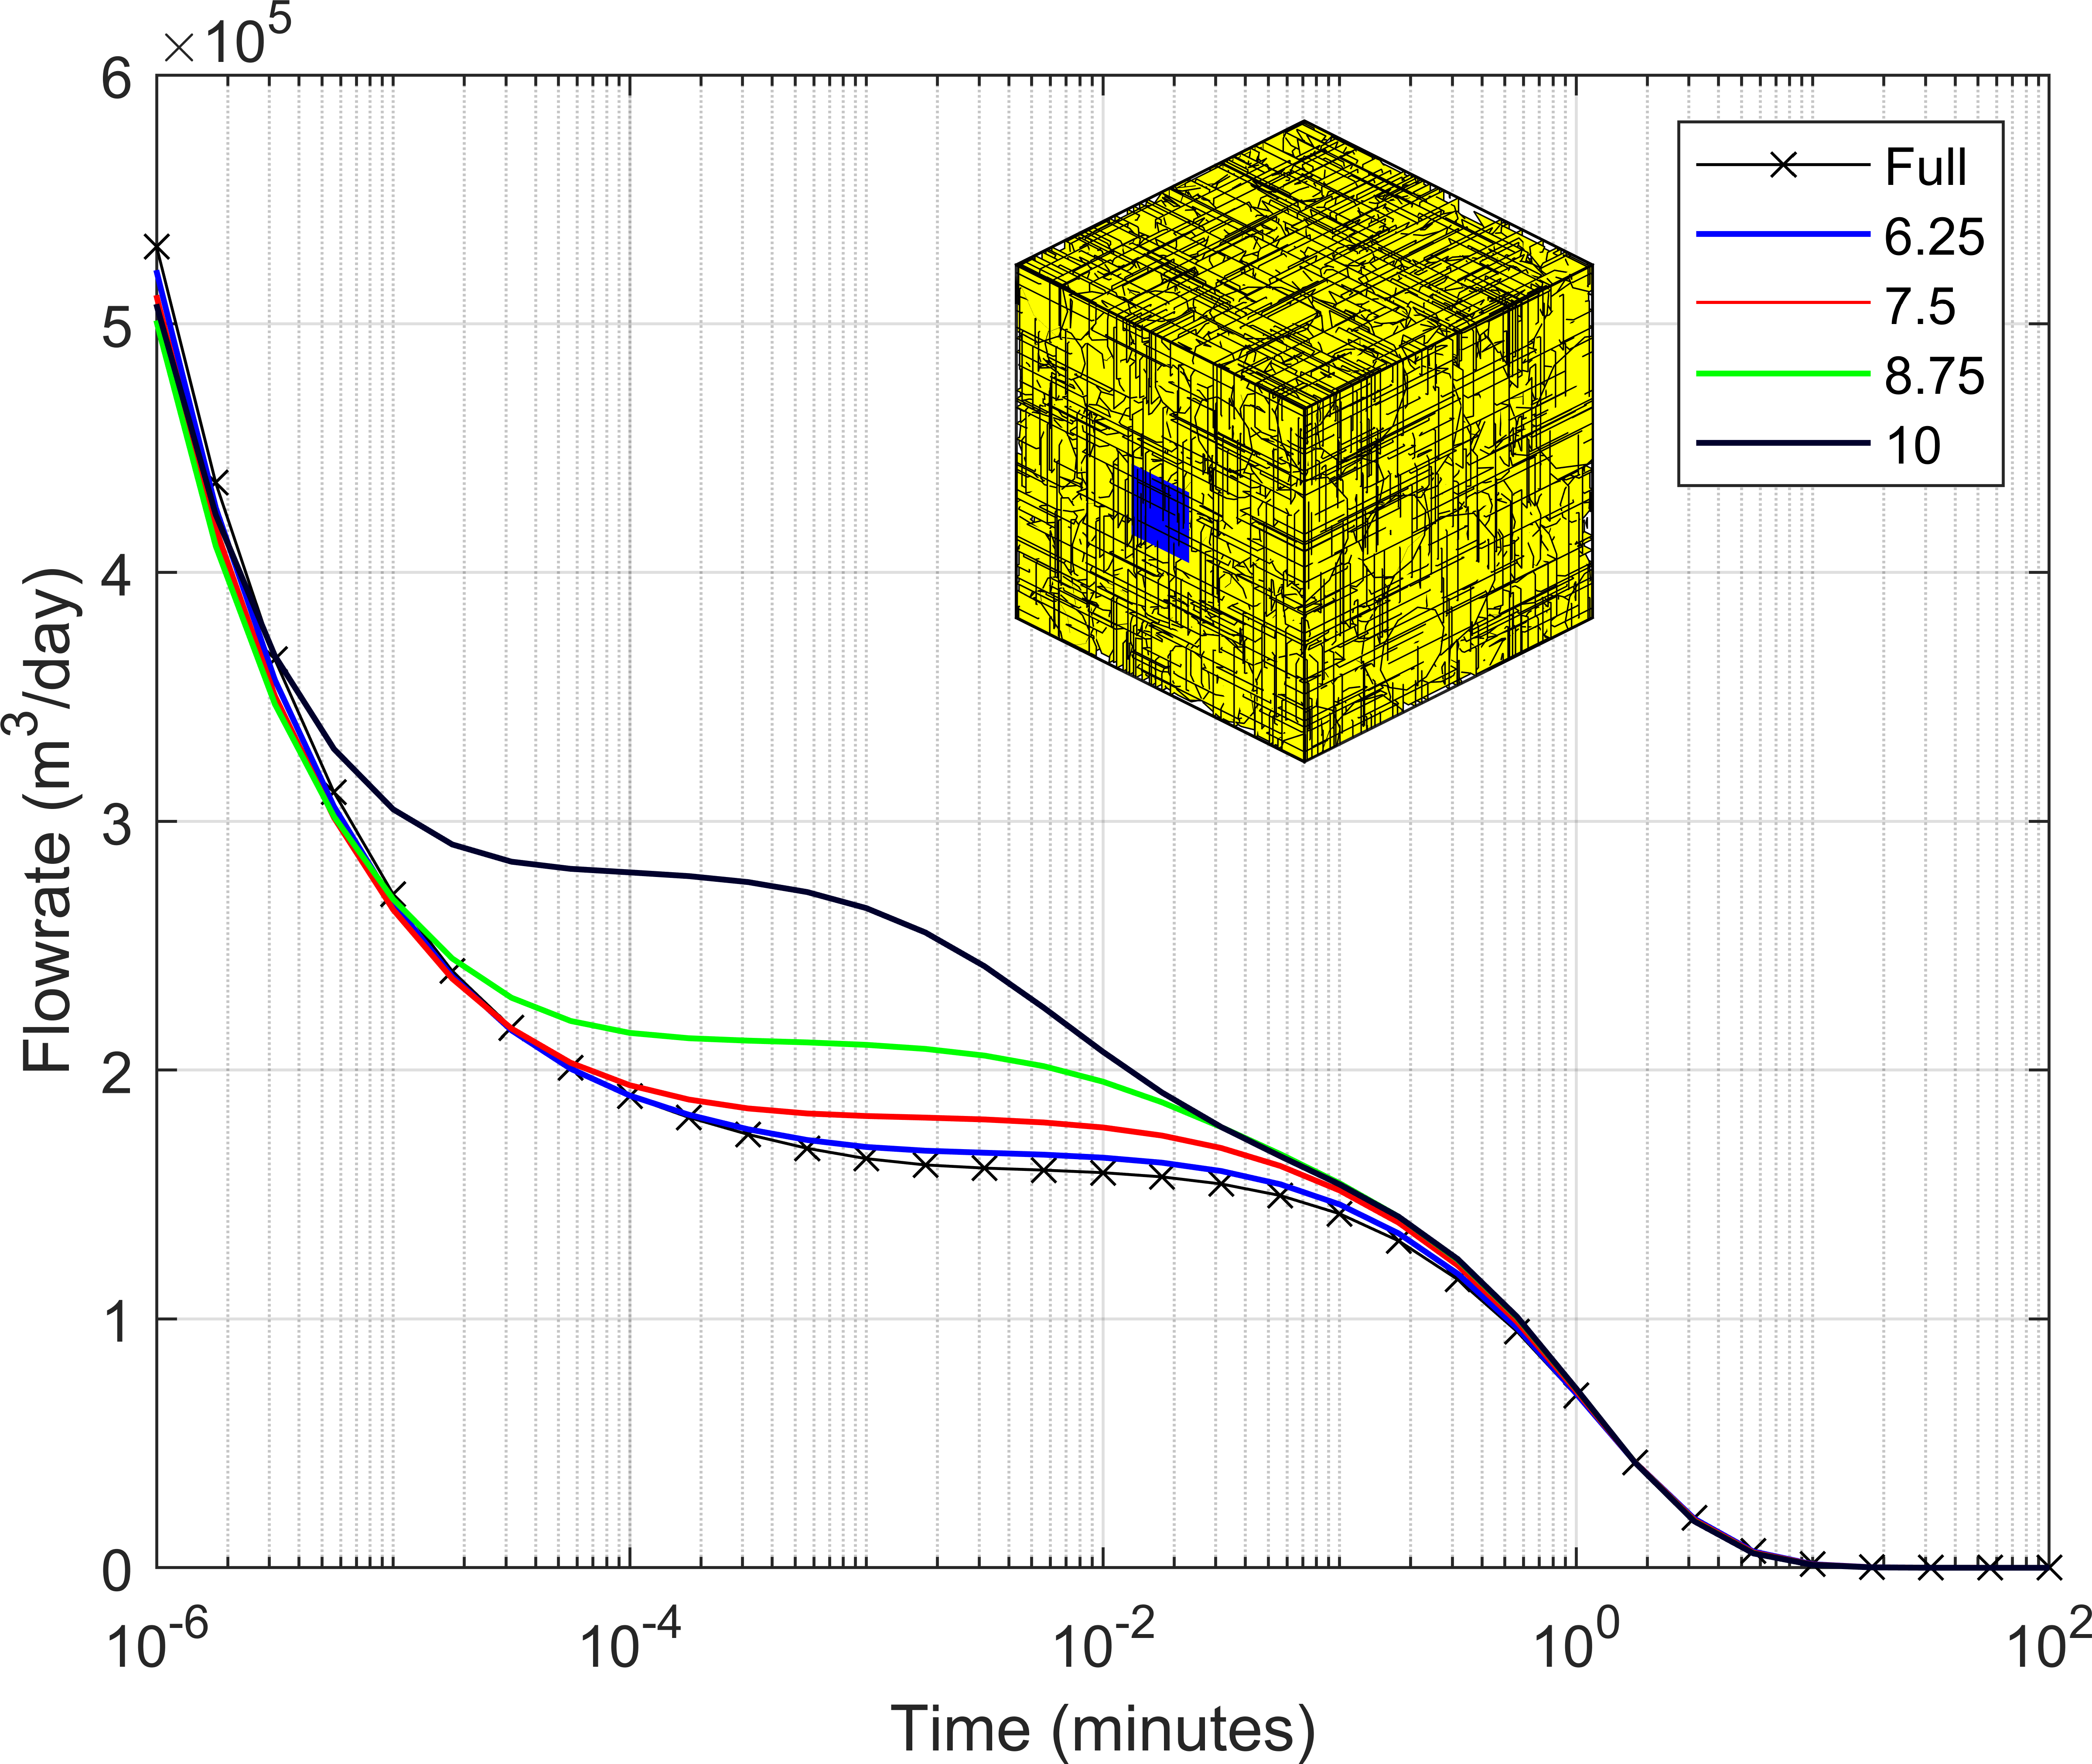
\includegraphics[width=\textwidth]{DD_main/Plot_Drawdown_Case_03_BCinset.png}
			\subcaption{Case B: 2x Density}
			\label{fig:DD_B}
		\end{subfigure}
		\begin{subfigure}{0.3\textwidth}
			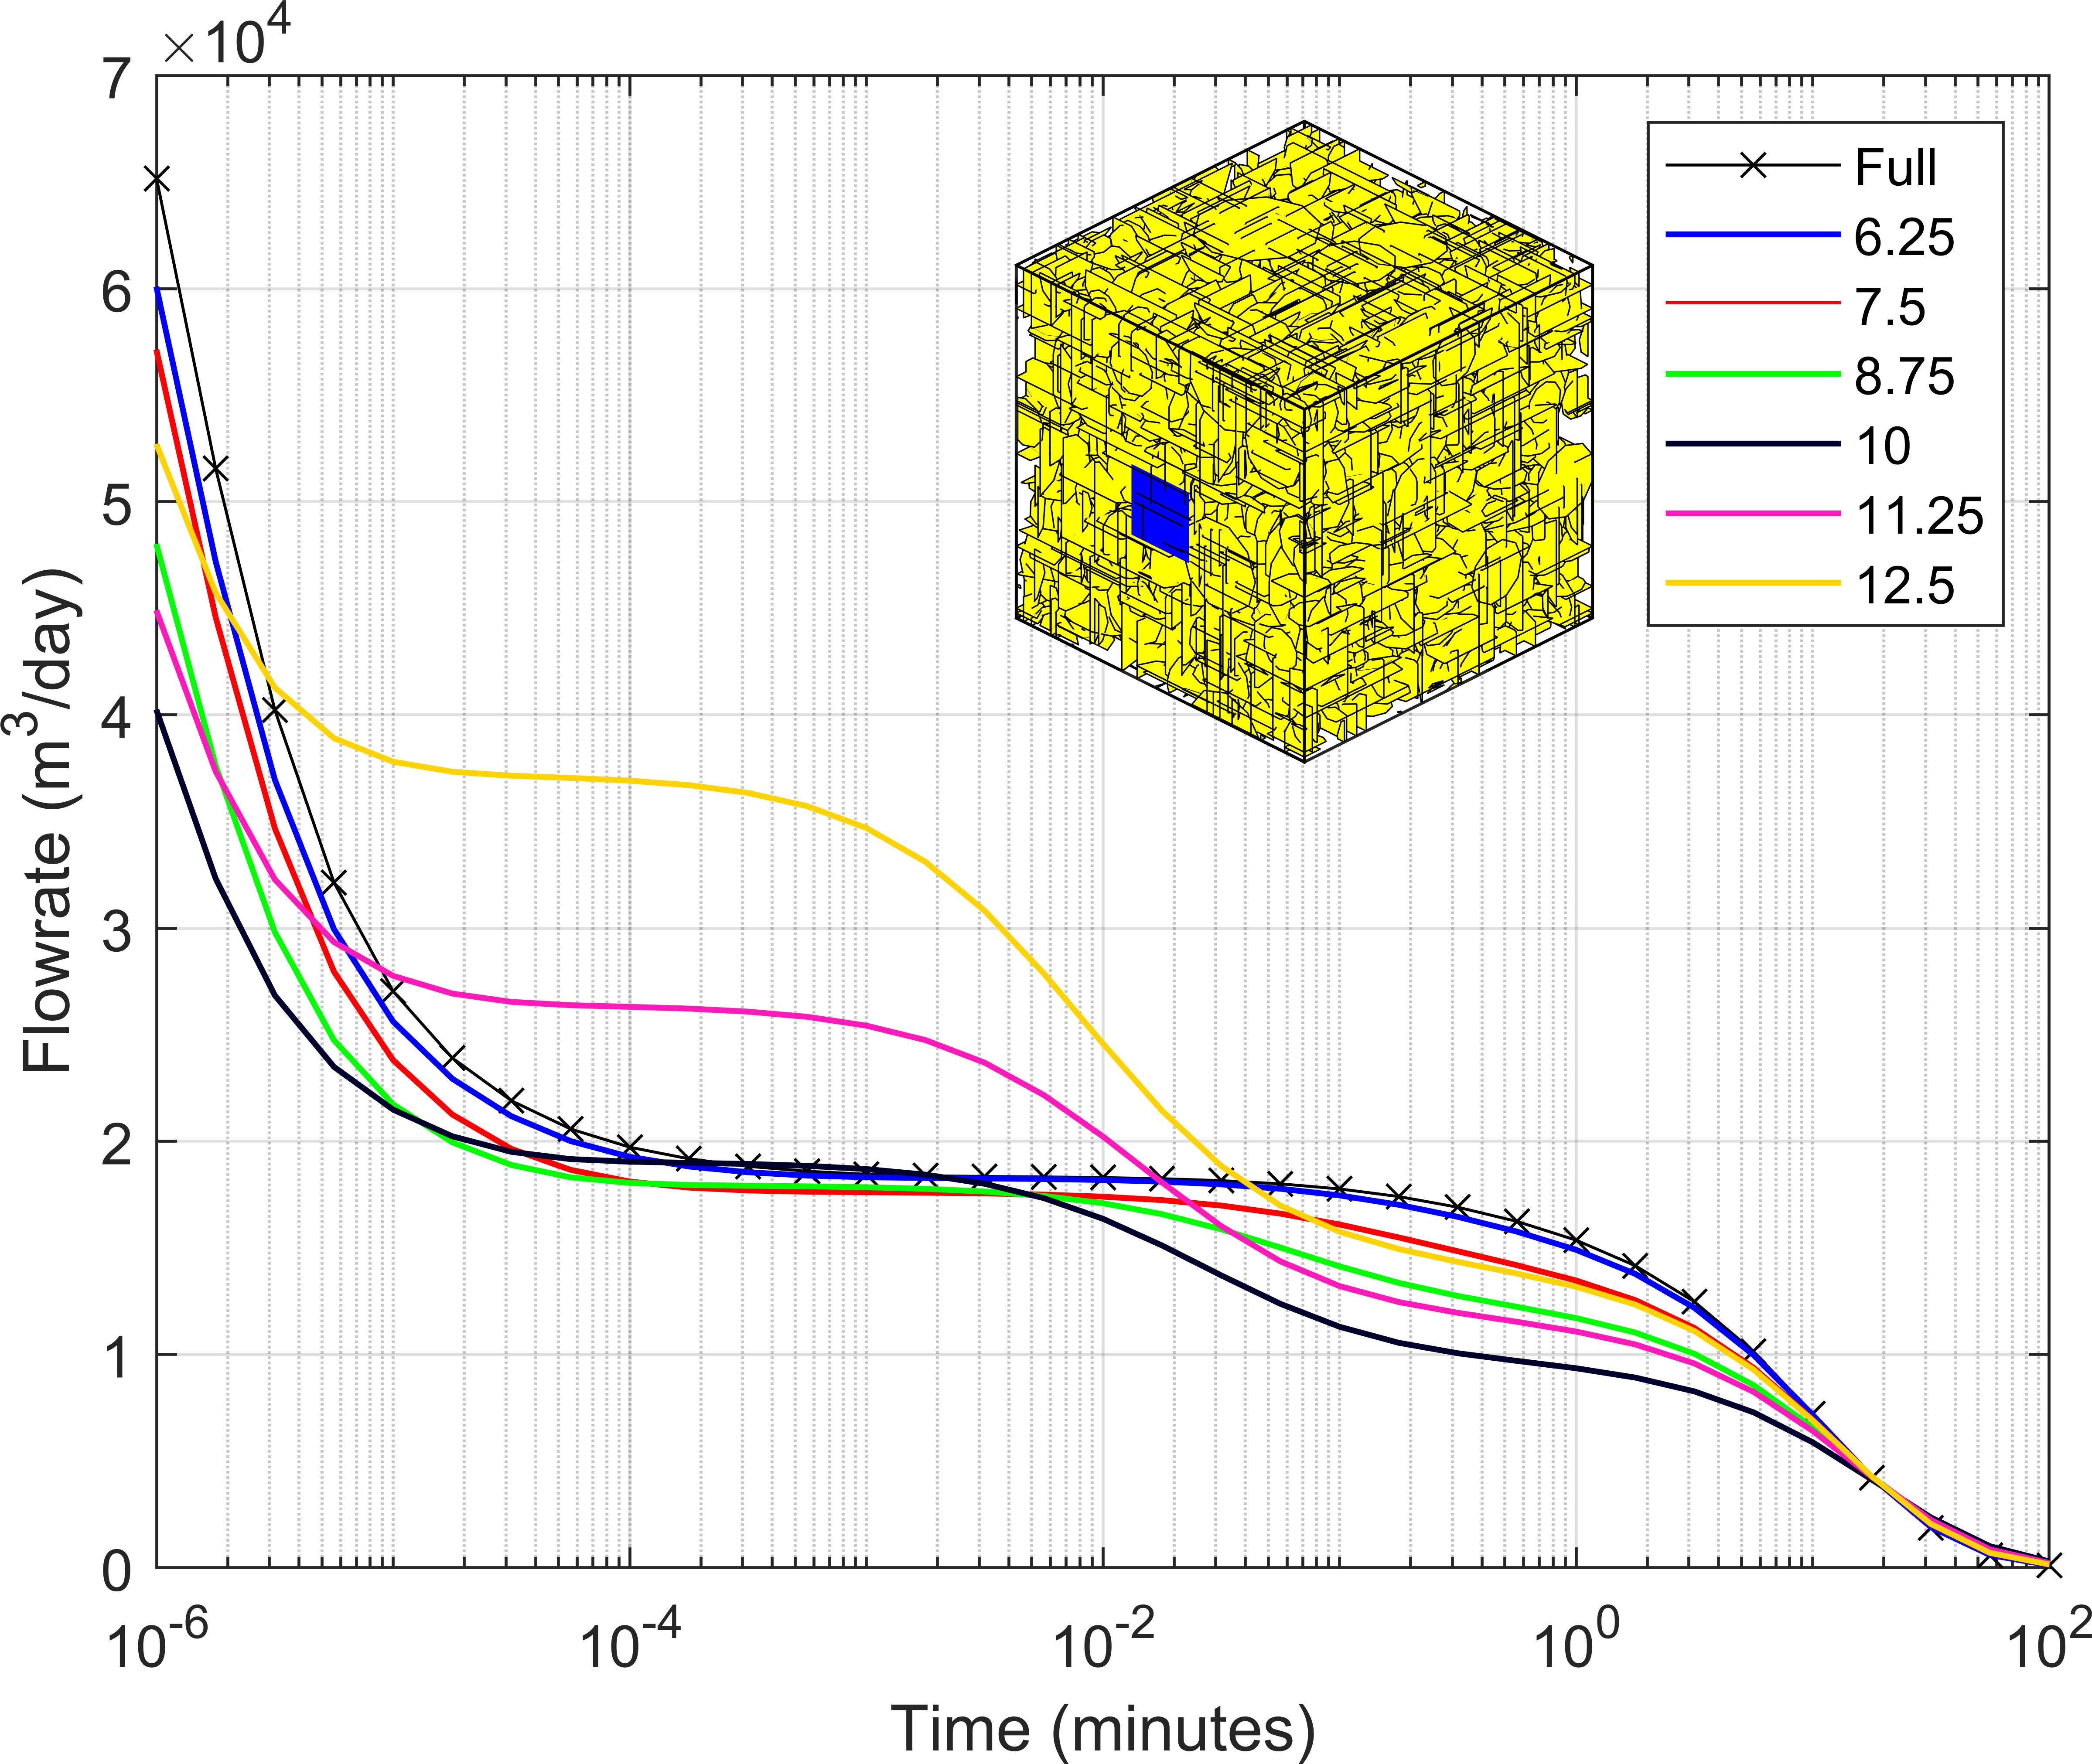
\includegraphics[width=\textwidth]{DD_main/Plot_Drawdown_Case_05_BCinset.png}
			\subcaption{Case C: 2x Size Exponent}
			\label{fig:DD_C}
		\end{subfigure}
		\\
		\begin{subfigure}{0.3\textwidth}
			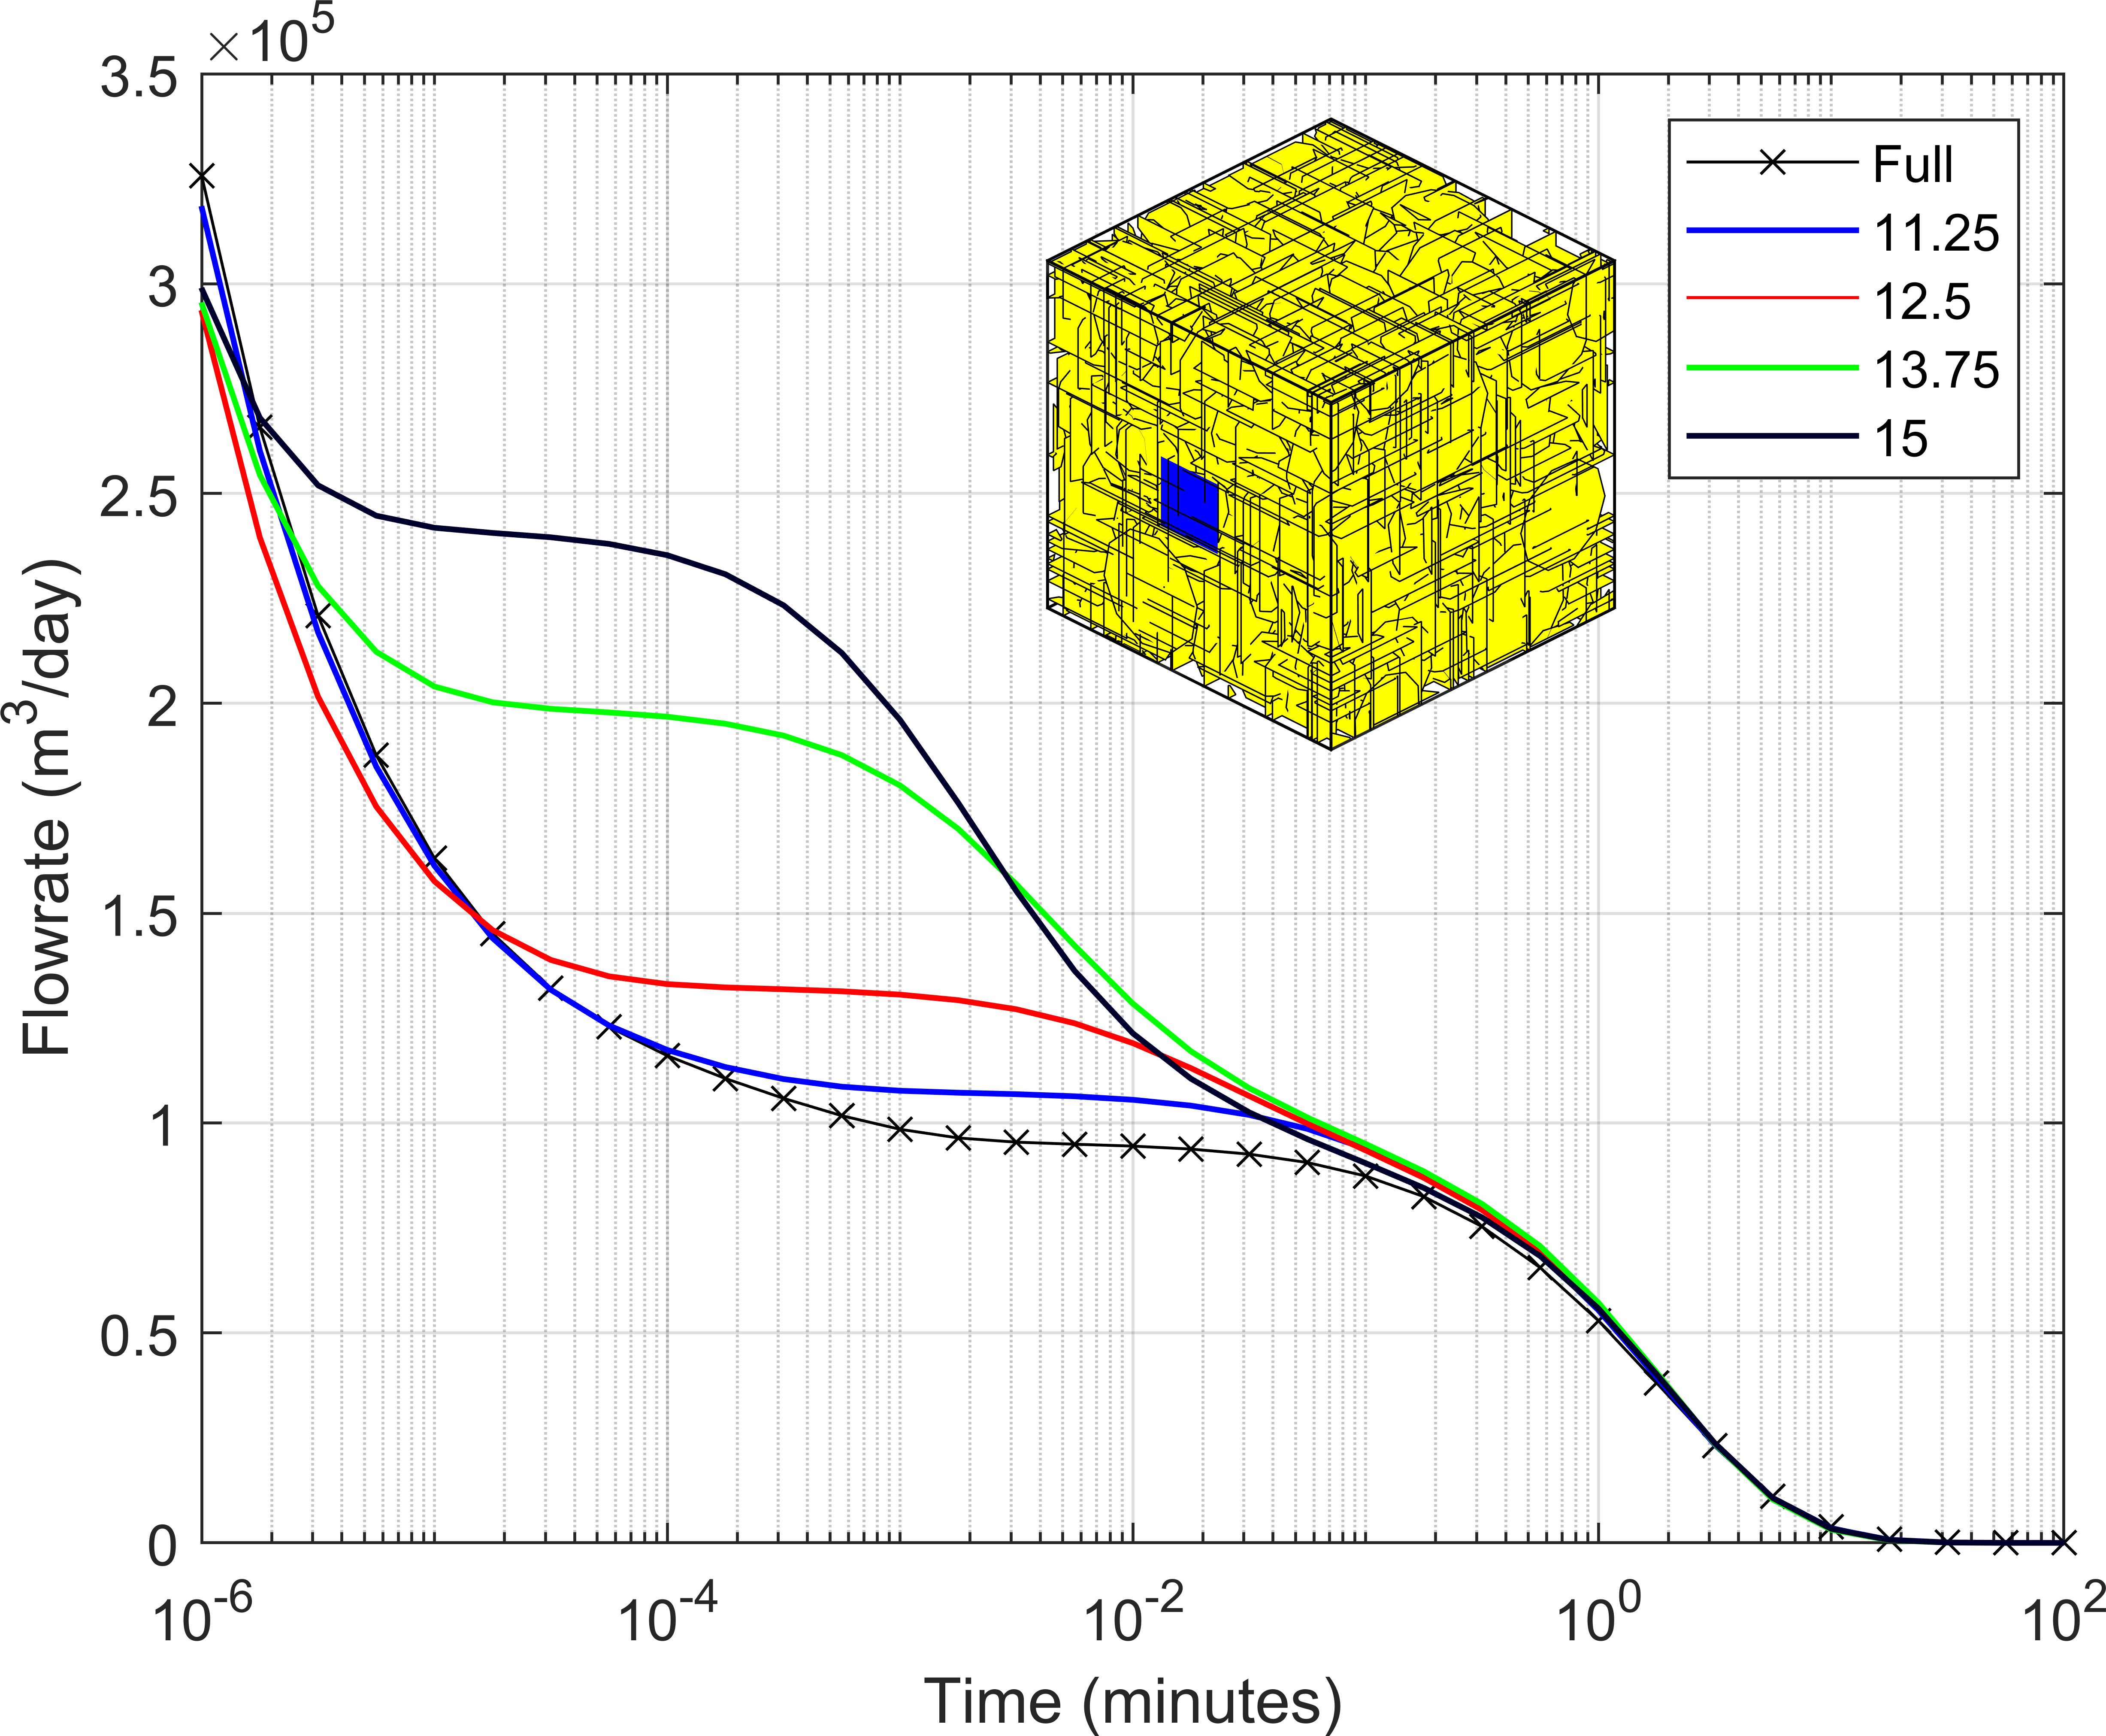
\includegraphics[width=\textwidth]{DD_main/Plot_Drawdown_Case_07_BCinset.png}
			\subcaption{Case D: 2x Min Size}
			\label{fig:DD_D}
		\end{subfigure}
		\begin{subfigure}{0.3\textwidth}
			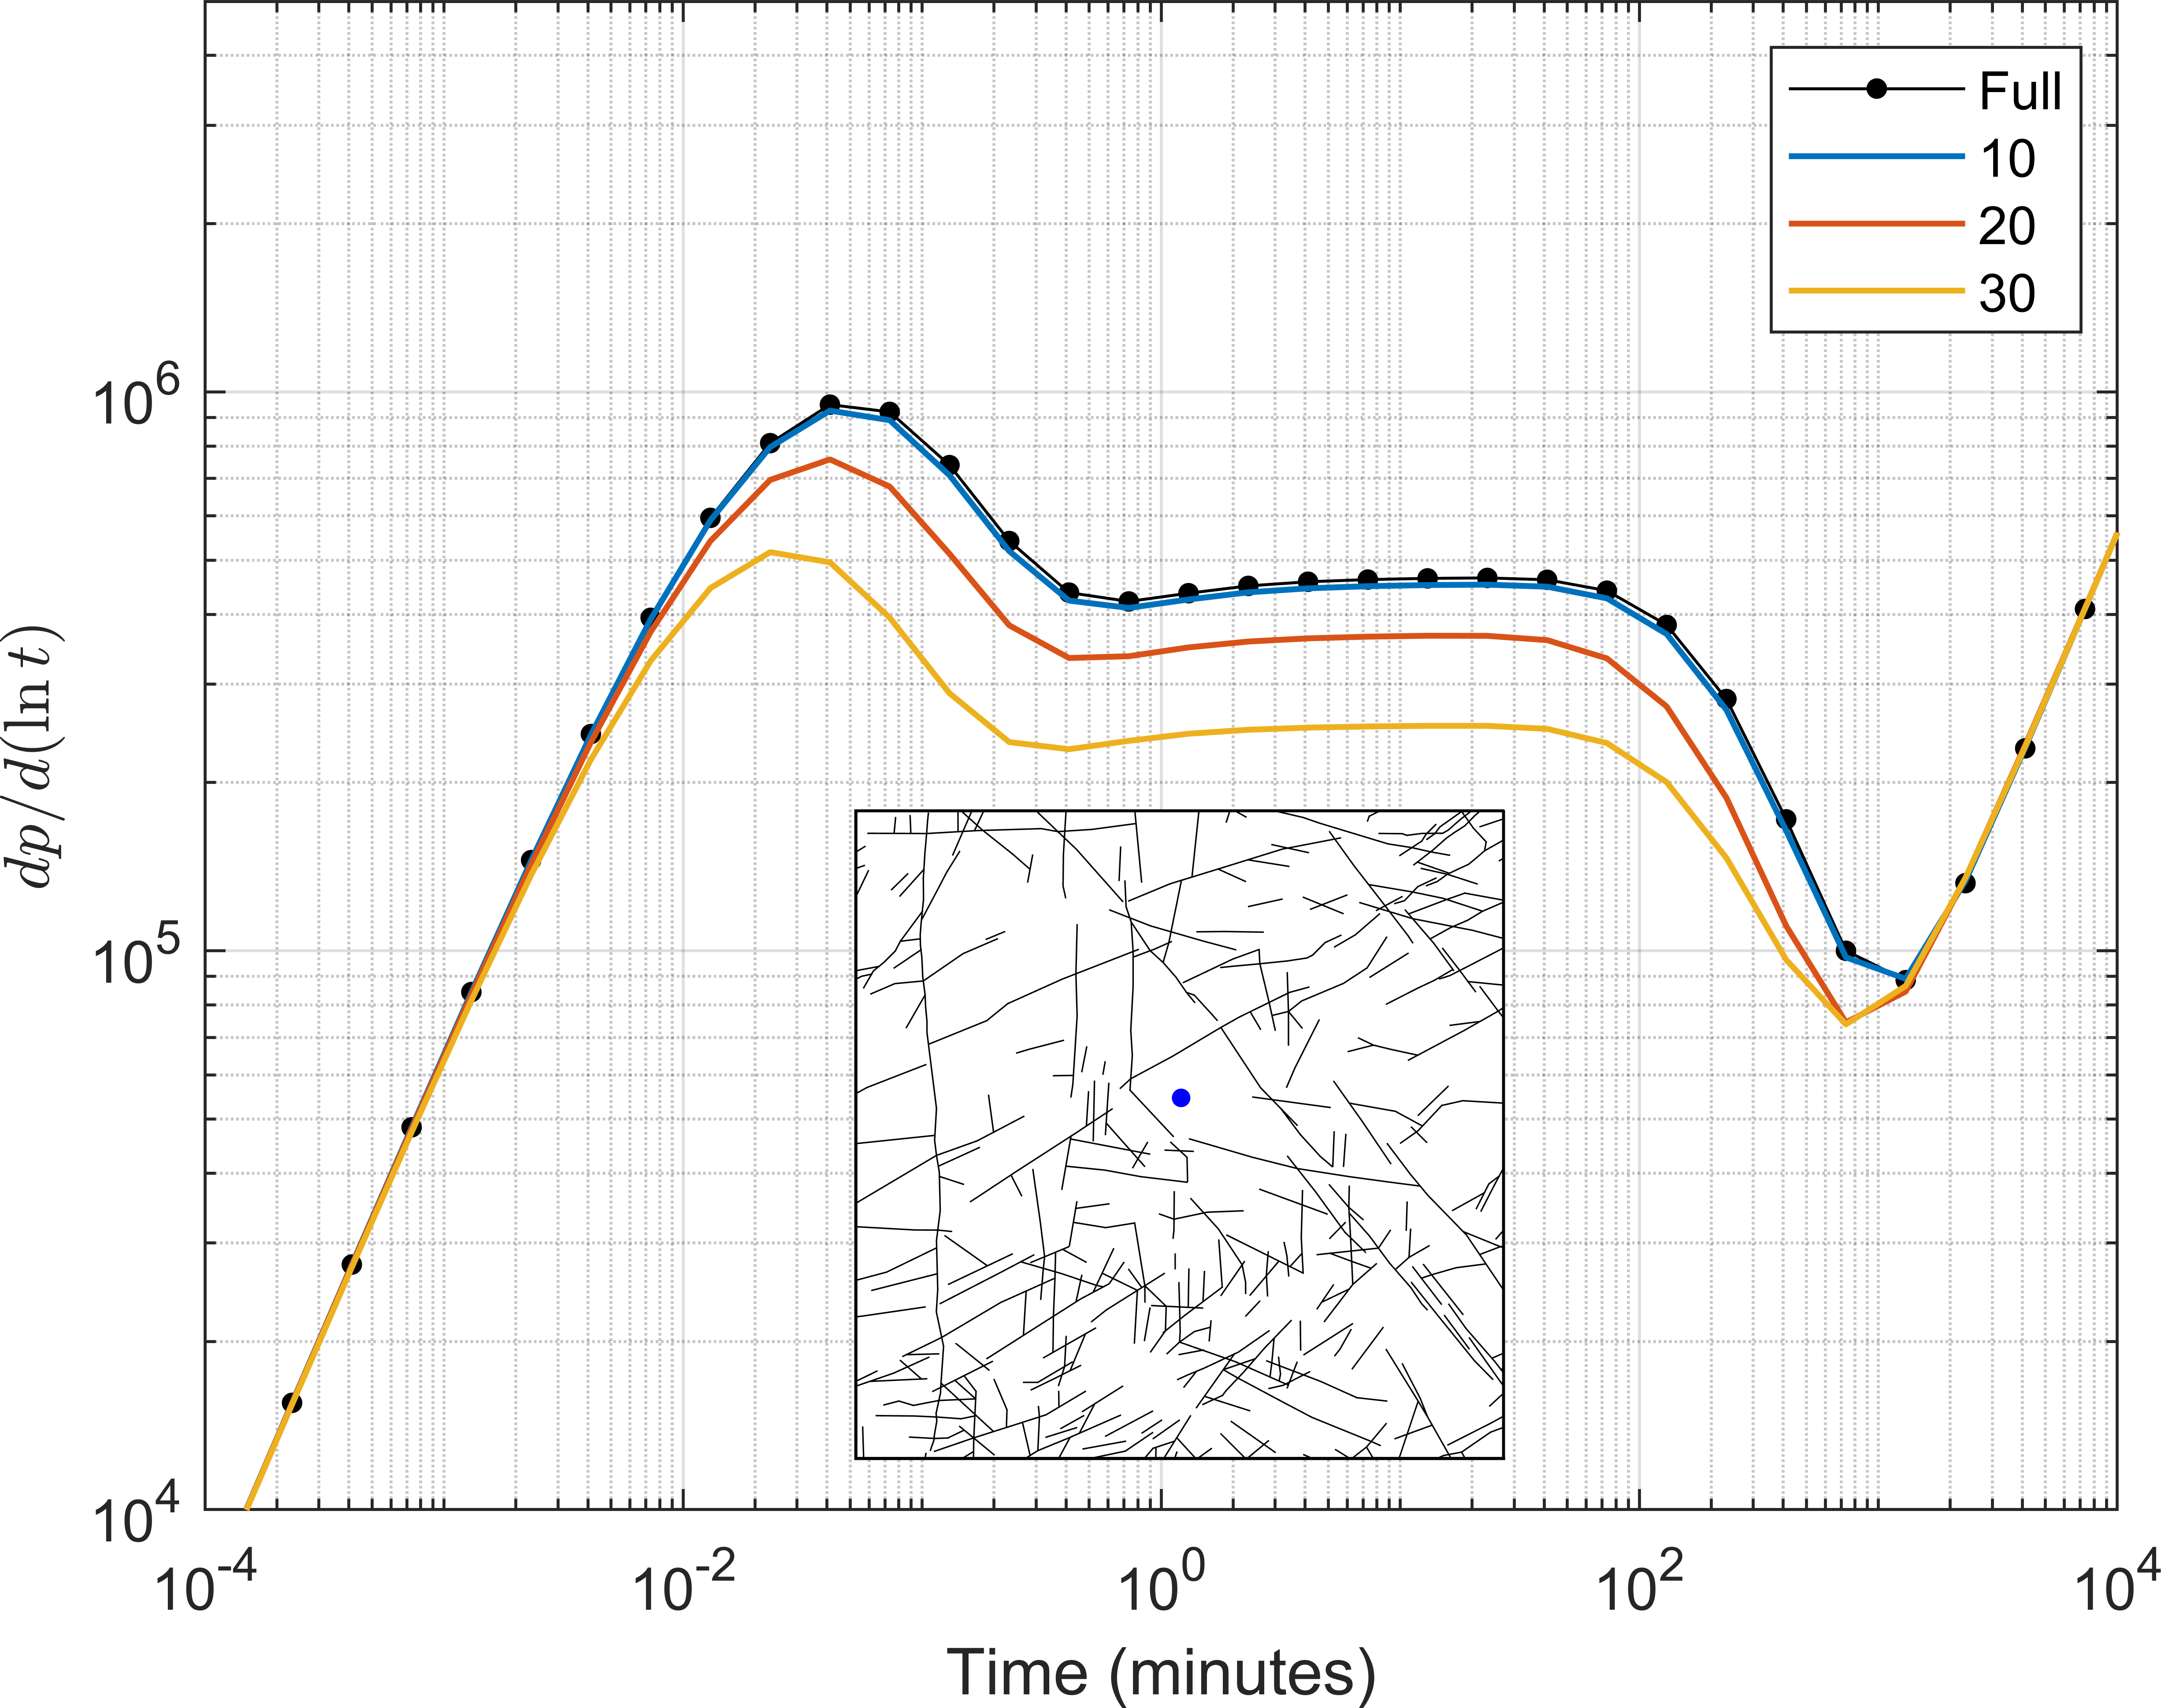
\includegraphics[width=\textwidth]{DD_main/Apodi2_matwell_BCinset.png}
			\subcaption{Apodi 2}
			\label{fig:DD_A2}
		\end{subfigure}
		\begin{subfigure}{0.3\textwidth}
			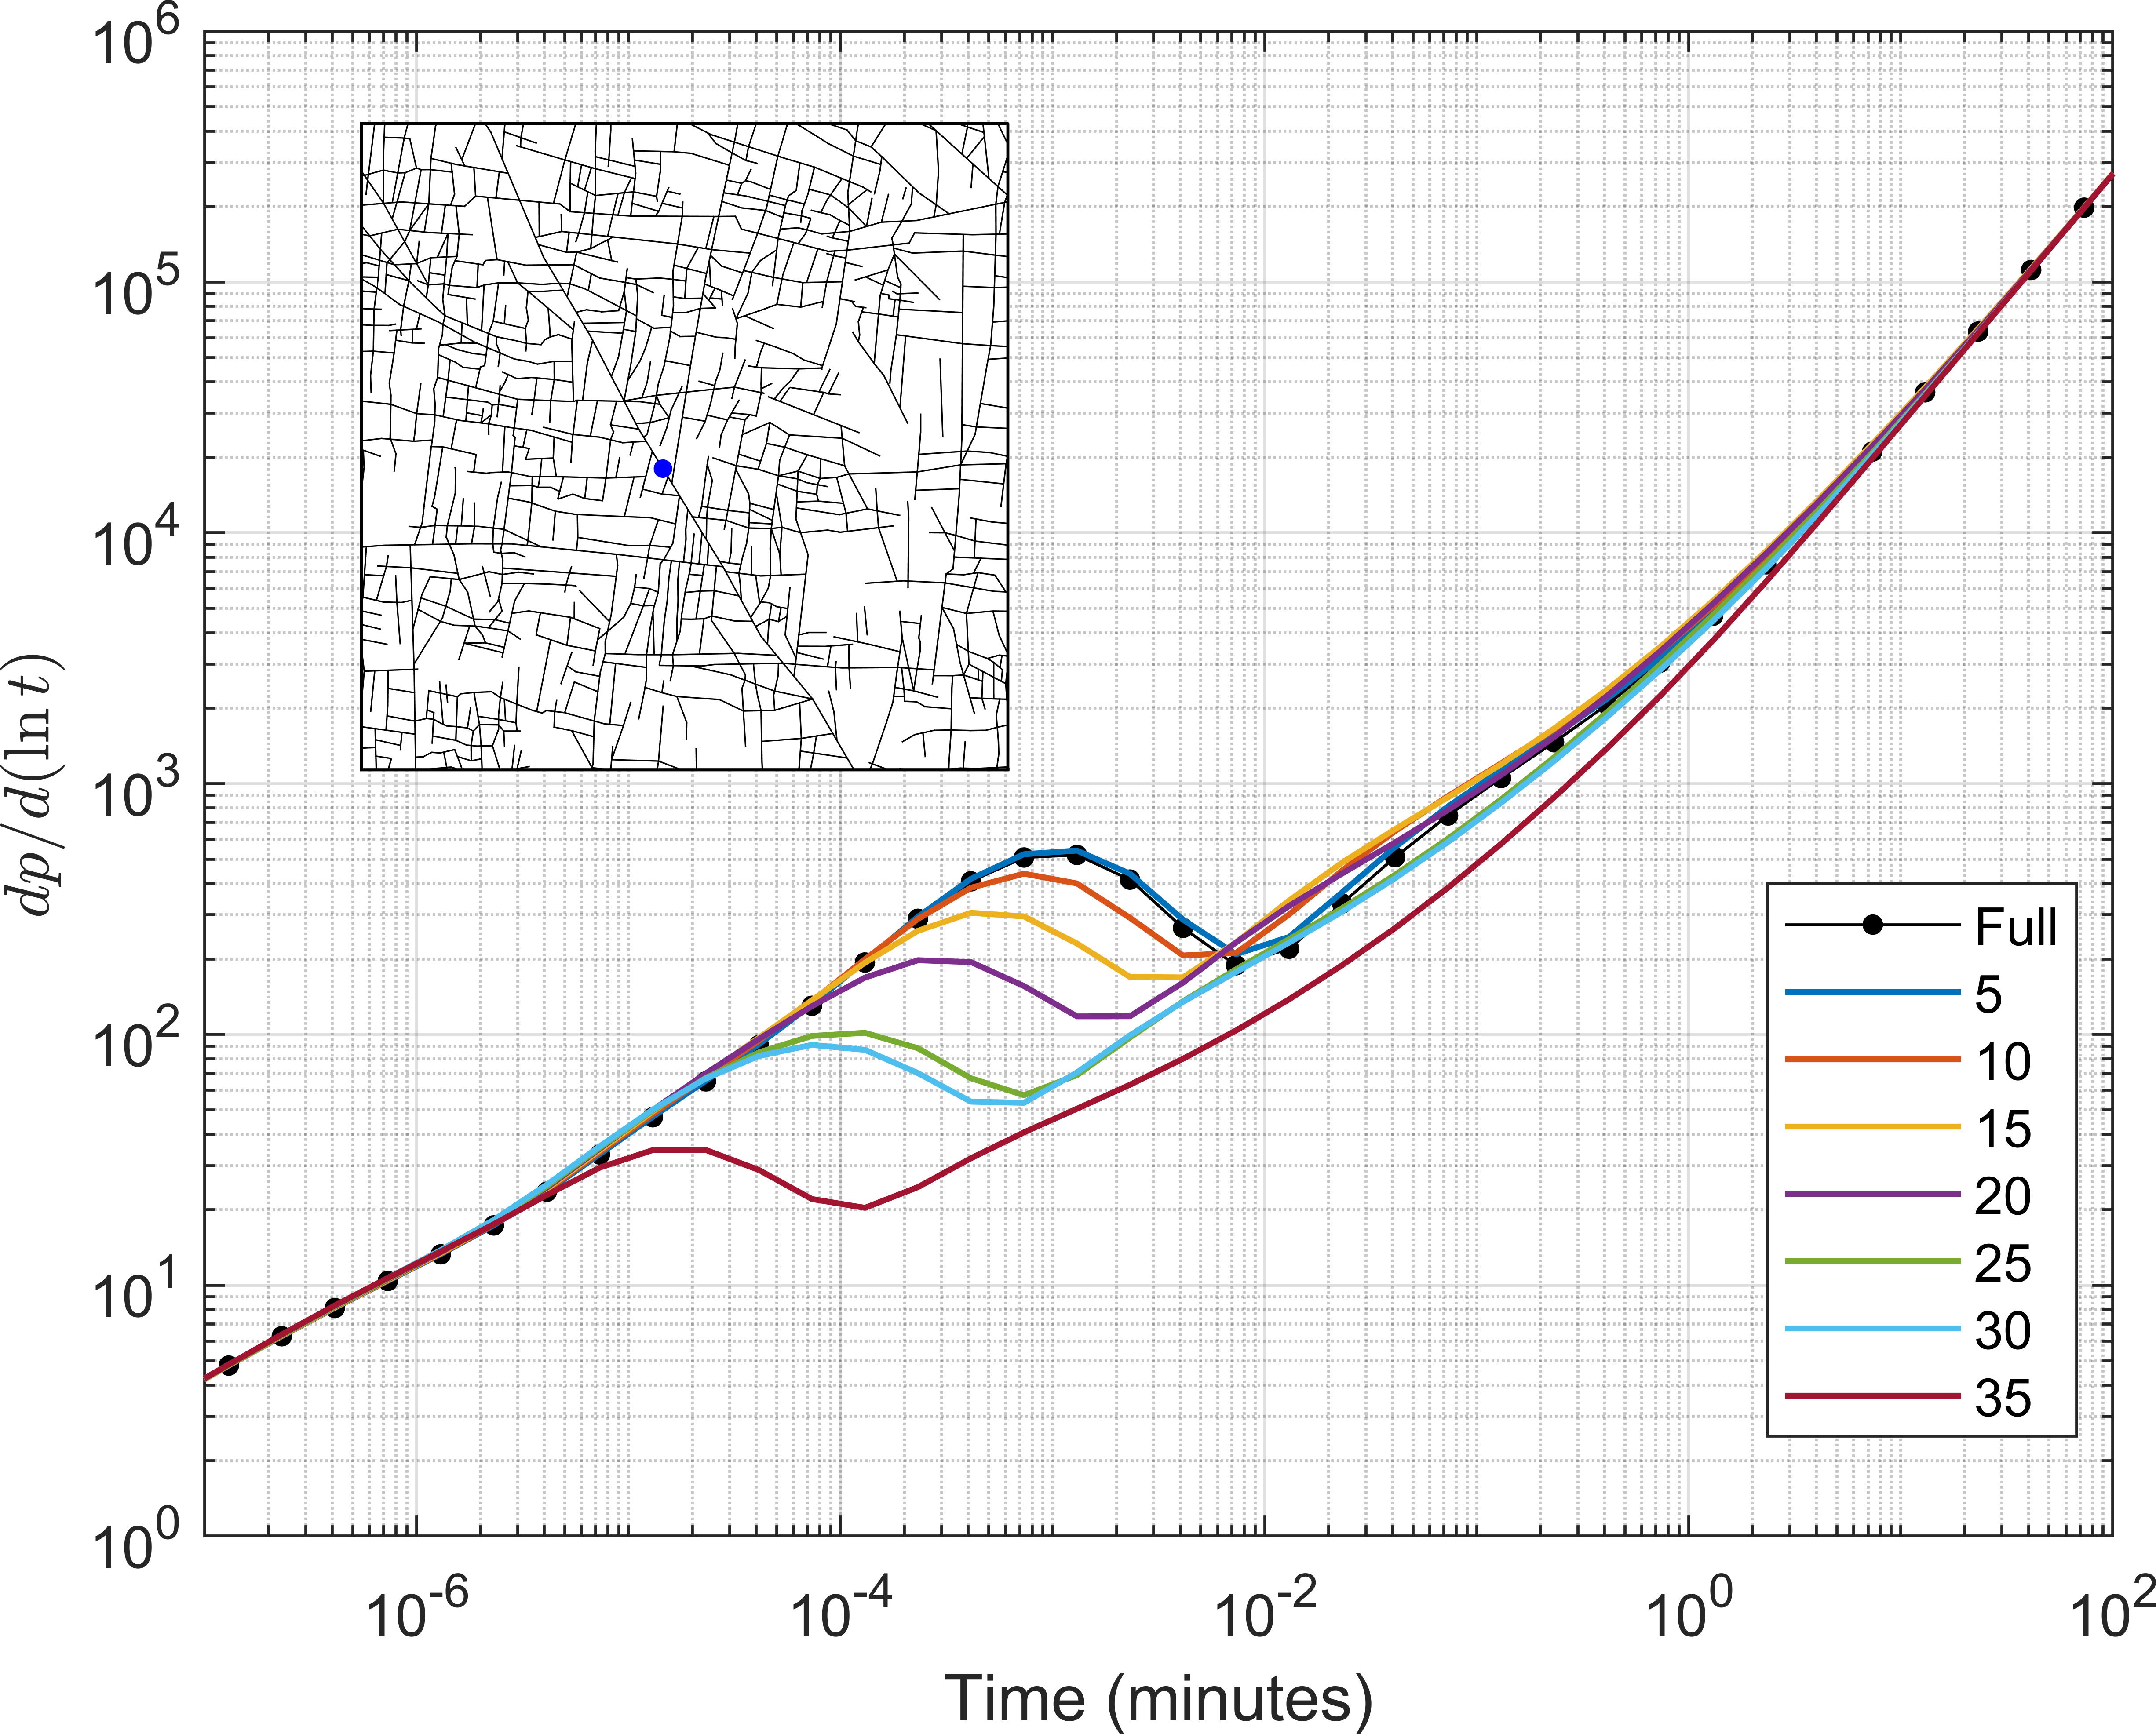
\includegraphics[width=\textwidth]{DD_main/Apodi4_fracwell_BCinset.png}
			\subcaption{Apodi 4}
			\label{fig:DD_A4}
		\end{subfigure}
		\caption{Drawdown curves for fully resolve models, and hybrid models corresponding to different partitioning sizes. (a)-(d) One full DFN realization is used per case. Fixed pressure is applied on blue faces. Domain size is 100m x 100m x 100m in all cases. (e)-(f) Fixed flowrate is applied at locations marked with blue circle. Domain size is 220m x 220m x 1m and 100m x 100m x 1m for Apodi 2 and 4 respectively.}
		\label{fig:DD}
	\end{figure}
	
	
	
\end{document}